\documentclass[a4paper,11pt]{article}
\usepackage[T1]{fontenc}
\usepackage{lmodern,microtype}
\usepackage[left=22mm,right=22mm,top=21mm,bottom=22mm,headheight=13pt,headsep=5mm,footskip=10mm]{geometry}
\usepackage{graphicx,booktabs,tabularx,ragged2e,titlesec,multicol,tikz}
\usepackage[hidelinks]{hyperref}
\usetikzlibrary{arrows.meta,positioning}
\graphicspath{{figures/}{Evaluation/figures/}}

\hypersetup{pdftitle={CropScan XR: BTP Third Evaluation},pdfauthor={Bhargav M}}
\microtypesetup{expansion=false}
\linespread{1.04}
\setlength{\emergencystretch}{2em}
\setlength{\parindent}{0pt}
\setlength{\parskip}{5pt}
\setlength{\columnsep}{17pt}
\setlength{\multicolsep}{3pt}
\setlength{\textfloatsep}{10pt plus 2pt minus 2pt}
\setlength{\intextsep}{8pt plus 2pt minus 2pt}
\setlength{\tabcolsep}{6pt}
\renewcommand{\arraystretch}{1.22}
\setlength{\abovecaptionskip}{5pt}
\setlength{\belowcaptionskip}{2pt}
\renewcommand{\figurename}{Fig.}
\newcolumntype{L}{>{\RaggedRight\arraybackslash}X}
\newcolumntype{P}[1]{>{\RaggedRight\arraybackslash}p{#1}}
\newcolumntype{N}[1]{>{\RaggedLeft\arraybackslash}p{#1}}
\titleformat{\section}{\large\sffamily\bfseries}{\thesection}{0.65em}{\MakeUppercase}
\titlespacing*{\section}{0pt}{10pt}{4pt}
\titleformat{\subsection}{\normalsize\bfseries}{}{0pt}{}
\titlespacing*{\subsection}{0pt}{7pt}{2pt}

\newcommand{\tabhead}[1]{\leavevmode\textbf{#1}}
\newcommand{\smallnote}[1]{{\small #1\par}}
\newcommand{\panel}[2]{%
  \begin{minipage}[t]{.484\linewidth}
  \includegraphics[width=\linewidth]{#1}\par
  \vspace{1pt}{\small #2}
  \end{minipage}}
\makeatletter
\def\ps@paper{%
  \def\@oddhead{\hbox to\textwidth{\small CropScan XR\hfil BTP Third Evaluation}}%
  \let\@evenhead\@oddhead
  \def\@oddfoot{\hfil\small\thepage\hfil}\let\@evenfoot\@oddfoot}
\def\ps@titlepaper{%
  \let\@oddhead\@empty\let\@evenhead\@empty
  \def\@oddfoot{\hfil\small\thepage\hfil}\let\@evenfoot\@oddfoot}
\long\def\@makecaption#1#2{%
  \vskip\abovecaptionskip
  {\small\RaggedRight\textbf{#1.} #2\par}
  \vskip\belowcaptionskip}
\makeatother

\begin{document}
\pagestyle{paper}
\thispagestyle{titlepaper}
\RaggedRight

\begin{center}
{\sffamily\bfseries\fontsize{23}{27}\selectfont CropScan XR\par}
\vspace{2pt}
{\sffamily\bfseries\Large VR Plant Disease \& Treatment System\par}
\vspace{8pt}
{\large\textbf{Bhargav M} \quad S20230030371\par}
\vspace{3pt}
{\small B.Tech Project, Third Evaluation \quad\textbar\quad 24 November 2026\par}
{\small Mentor: Dr. Pavan Kumar B N\par}
\end{center}

\begin{figure}[!ht]\centering
\panel{farm-gallery.jpg}{(a) Selecting a crop in the Farm}\hfill
\panel{leaf.jpg}{(b) Inspecting an affected leaf in the Lab}
\caption{The Unity experience gives learners a plant to find and a leaf to examine before they enter the Treatment Lab.}\label{fig:opening}
\end{figure}

\noindent\textbf{Abstract.}
CropScan XR is a team project that links a leaf-photo scanner to a plant disease lesson in virtual reality. I built the Unity experience, including the Farm, Lab and Treatment Lab, and a timeline that shows six weeks of simulated recovery. A teammate developed the backend. When the scanner identifies a supported case, the learner can find the matching plant in Unity, examine the leaf, try a guided treatment and see the simulated outcome. The lesson can also run offline. All 167 tests in a targeted Unity EditMode run passed, and I completed the inspection, treatment and recovery workflow on a Meta Quest headset. In the team's classifier benchmark, BioCLIP v6 achieved 77.1\% top-1 accuracy on PlantDoc field photos and 99.4\% on PlantVillage lab photos. A learner study could test whether the finished prototype helps people recognise symptoms or choose an appropriate response.

\noindent\textbf{Index Terms.} Virtual reality, plant disease recognition, interactive training, Unity.

\begin{multicols}{2}
\section{Introduction}
Plant pests and diseases account for a substantial share of crop losses \cite{fao}. A leaf photo can help narrow down the possibilities, but different conditions can leave similar marks. Field photos add variation in lighting, background and angle. Earlier work on PlantVillage shows how a classifier trained on controlled images can lose accuracy on other photographs \cite{mohanty}.

\columnbreak
CropScan XR connects the scanner's result to a lesson. I wanted learners to follow the same specimen from the Farm to the Lab, look closely at its symptoms and try a treatment before reviewing the outcome. The recovery timeline uses six illustrative weekly stages. Each stage shows an example for training.
\end{multicols}

\clearpage
\section{Related Work}
The literature gives CropScan XR two points of comparison. The image-classification studies show why field photos need a separate benchmark. The VR studies show how researchers have used immersive environments for plant assessment and training.

\begin{table}[!ht]
\caption{Related work in plant disease recognition and immersive plant learning.}\label{tab:lit}
\vspace{3pt}
\begin{tabularx}{\linewidth}{@{}P{.20\linewidth}LL@{}}
\toprule
\tabhead{Study} & \tabhead{What the authors examined} & \tabhead{Relevance to CropScan XR}\\
\midrule
Mohanty et al. \cite{mohanty} & Classified leaf images from PlantVillage and tested transfer beyond controlled photographs. & Explains why the team reports lab and field scores separately.\\
\addlinespace[3pt]
Singh et al. \cite{plantdoc} & Introduced PlantDoc, which includes plant disease images from less controlled settings. & Provides the field benchmark used in the team results.\\
\addlinespace[3pt]
Sakha et al. \cite{sakha} & Used 3D reconstructions from field scans so breeders could compare plant traits in VR. & Shows how VR can support close inspection and comparison of plant specimens.\\
\addlinespace[3pt]
Bondesan et al. \cite{bondesan} & Compared VR and slideshow lessons that taught students to judge vine vigour. & Offers an example of evaluating learning with a separate task after training.\\
\addlinespace[3pt]
Cheng \cite{cheng} & Studied how teachers and pupils used an immersive environment to learn about plants. & Provides context for a plant lesson built around observation and interaction.\\
\addlinespace[3pt]
Stevens et al. \cite{bioclip} & Developed BioCLIP, a pretrained model for recognizing biological images. & Supplies the visual backbone for the team's current classifier.\\
\bottomrule
\end{tabularx}
\end{table}

\subsection*{Where this project fits}
The plant assessment systems above focus on examining traits, and the image classifiers focus on identifying a condition. CropScan XR connects a supported scan to a short treatment exercise. The learner sees the symptoms on a specific specimen, makes a choice in the Treatment Lab and then reviews the simulated recovery. PlantWild supported earlier field experiments \cite{plantwild}, and EfficientNet-B0 served as the team's original baseline \cite{eff}.

\section{Progress Since the Previous Evaluation}
For my previous evaluation, I presented a 360-degree VR movie player. In CropScan XR, I moved from video playback to a scene where learners can choose a plant and interact with it.

My mentor asked the team to connect leaf-photo identification with a VR lesson that shows treatment and recovery. My teammate developed the scanner backend. I built the scenes and interactions in Unity, added the six-week timeline, and tested the experience on Quest.

\clearpage
\section{Methodology}
The connected workflow starts with a leaf photo. The offline workflow starts with a case selected inside Unity. Both lead to the same inspection and treatment steps.

\begin{figure}[!ht]\centering
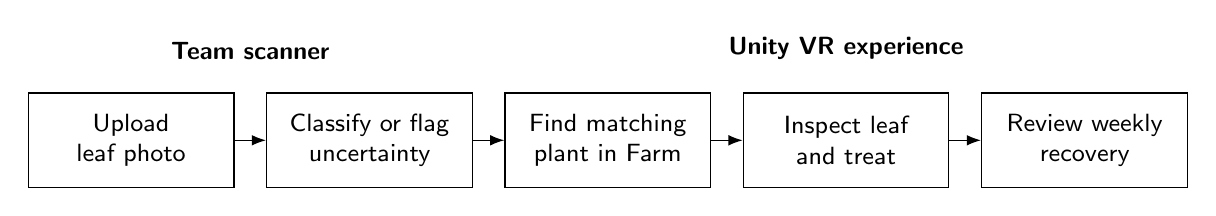
\begin{tikzpicture}[
  font=\sffamily\small,
  stage/.style={draw=black,line width=.45pt,align=center,text width=24mm,
    minimum height=12mm,inner xsep=3pt,inner ysep=3pt},
  flow/.style={-{Latex[length=1.8mm]},draw=black,line width=.45pt},
  node distance=4mm]
\node[stage] (photo) {Upload\\leaf photo};
\node[stage,right=of photo] (predict) {Classify or flag\\uncertainty};
\node[stage,right=of predict] (farm) {Find matching\\plant in Farm};
\node[stage,right=of farm] (lab) {Inspect leaf\\and treat};
\node[stage,right=of lab] (review) {Review weekly\\recovery};
\node[font=\sffamily\small\bfseries,anchor=south] at ([xshift=2mm,yshift=3mm]photo.north east) {Team scanner};
\node[font=\sffamily\small\bfseries,anchor=south] at ([yshift=3mm]lab.north) {Unity VR experience};
\draw[flow] (photo)--(predict);
\draw[flow] (predict)--(farm);
\draw[flow] (farm)--(lab);
\draw[flow] (lab)--(review);
\end{tikzpicture}
\caption{Connected workflow. The arrow into Unity applies when the prediction maps to a supported VR case.}\label{fig:workflow}
\end{figure}

\begin{multicols}{2}
\subsection*{A. Photo to prediction}
A teammate's FastAPI backend prepares a $224\times224$ RGB input and runs the BioCLIP-derived model with ONNX Runtime. It can flag an uncertain result based on confidence, image detail or a non-leaf prediction. A successful result can show the predicted class, confidence score and a visual overlay of the areas that influenced the prediction.

\subsection*{B. Prediction to specimen}
A supported result maps to a crop, disease and specimen. The scan ID points to the photograph, the session ID keeps track of the run and the specimen ID identifies the plant in Unity. The Windows launcher passes the scan ID to the Unity app. The XR rig stays active while Unity switches between scenes.

\columnbreak
\subsection*{C. Treatment exercise}
The learner inspects the affected leaf, moves into the Treatment Lab and adjusts the scenario controls for temperature, fertiliser, training spray and soil moisture. \emph{Apply} records the inputs. \emph{Check Health} assesses them against the selected scenario and gives feedback.

\subsection*{D. Recovery review}
The learner can step through six simulated weeks and compare the plant's appearance with its starting condition. A connected session keeps the same lesson rules when it resumes. The offline path uses SQLite to store the lesson and progress locally.
\end{multicols}

\begin{figure}[!ht]\centering
\panel{lab-week-1.jpg}{(a) Week 1, before the simulated recovery}\hfill
\panel{lab-week-6.jpg}{(b) Week 6, after the simulated recovery}
\caption{Two stages of the tomato early blight lesson. The timeline shows how the scenario changes over six simulated weeks.}\label{fig:recovery}
\end{figure}

\clearpage
\section{Implementation Details}
I used Unity 6000.5.5f1 with OpenXR and the XR Interaction Toolkit. The Farm holds the specimens, the Lab presents the leaves and recovery timeline, and the Treatment Lab handles the controls and feedback. A persistent XR rig keeps the player's headset and controller input available as the scenes change.

\begin{table}[!ht]
\caption{Implementation stack and scope.}\label{tab:implementation}
\vspace{3pt}
\begin{tabularx}{\linewidth}{@{}P{.21\linewidth}LL@{}}
\toprule
\tabhead{Area} & \tabhead{Tools and targets} & \tabhead{What the system does}\\
\midrule
Unity VR & Unity, C\#, Universal Render Pipeline, OpenXR and XR Interaction Toolkit & Runs the Farm, Lab and Treatment scenes on Windows desktop and Meta Quest.\\
\addlinespace[3pt]
Plant assets & Blender, Unity prefabs and shaders & Displays crop models, disease-specific leaves and simulated recovery visuals. Distant plants use simpler geometry or billboards.\\
\addlinespace[3pt]
Lesson content & SQLite and scan-to-VR mapping & Provides 58 authored treatment cases across 19 crops. The connected case map has 24 entries.\\
\addlinespace[3pt]
Team scanner & React, Vite, FastAPI and ONNX Runtime & Returns predictions from BioCLIP v6. The model has 69 outputs across 20 crops, including a non-leaf output.\\
\bottomrule
\end{tabularx}
\end{table}

I used tomato early blight for the demo. The case map keeps the same specimen selected as the learner moves from the Farm to the Lab and Treatment Lab. The project repository contains the scenes, plant catalogue and treatment content \cite{repo}.

\begin{figure}[!ht]\centering
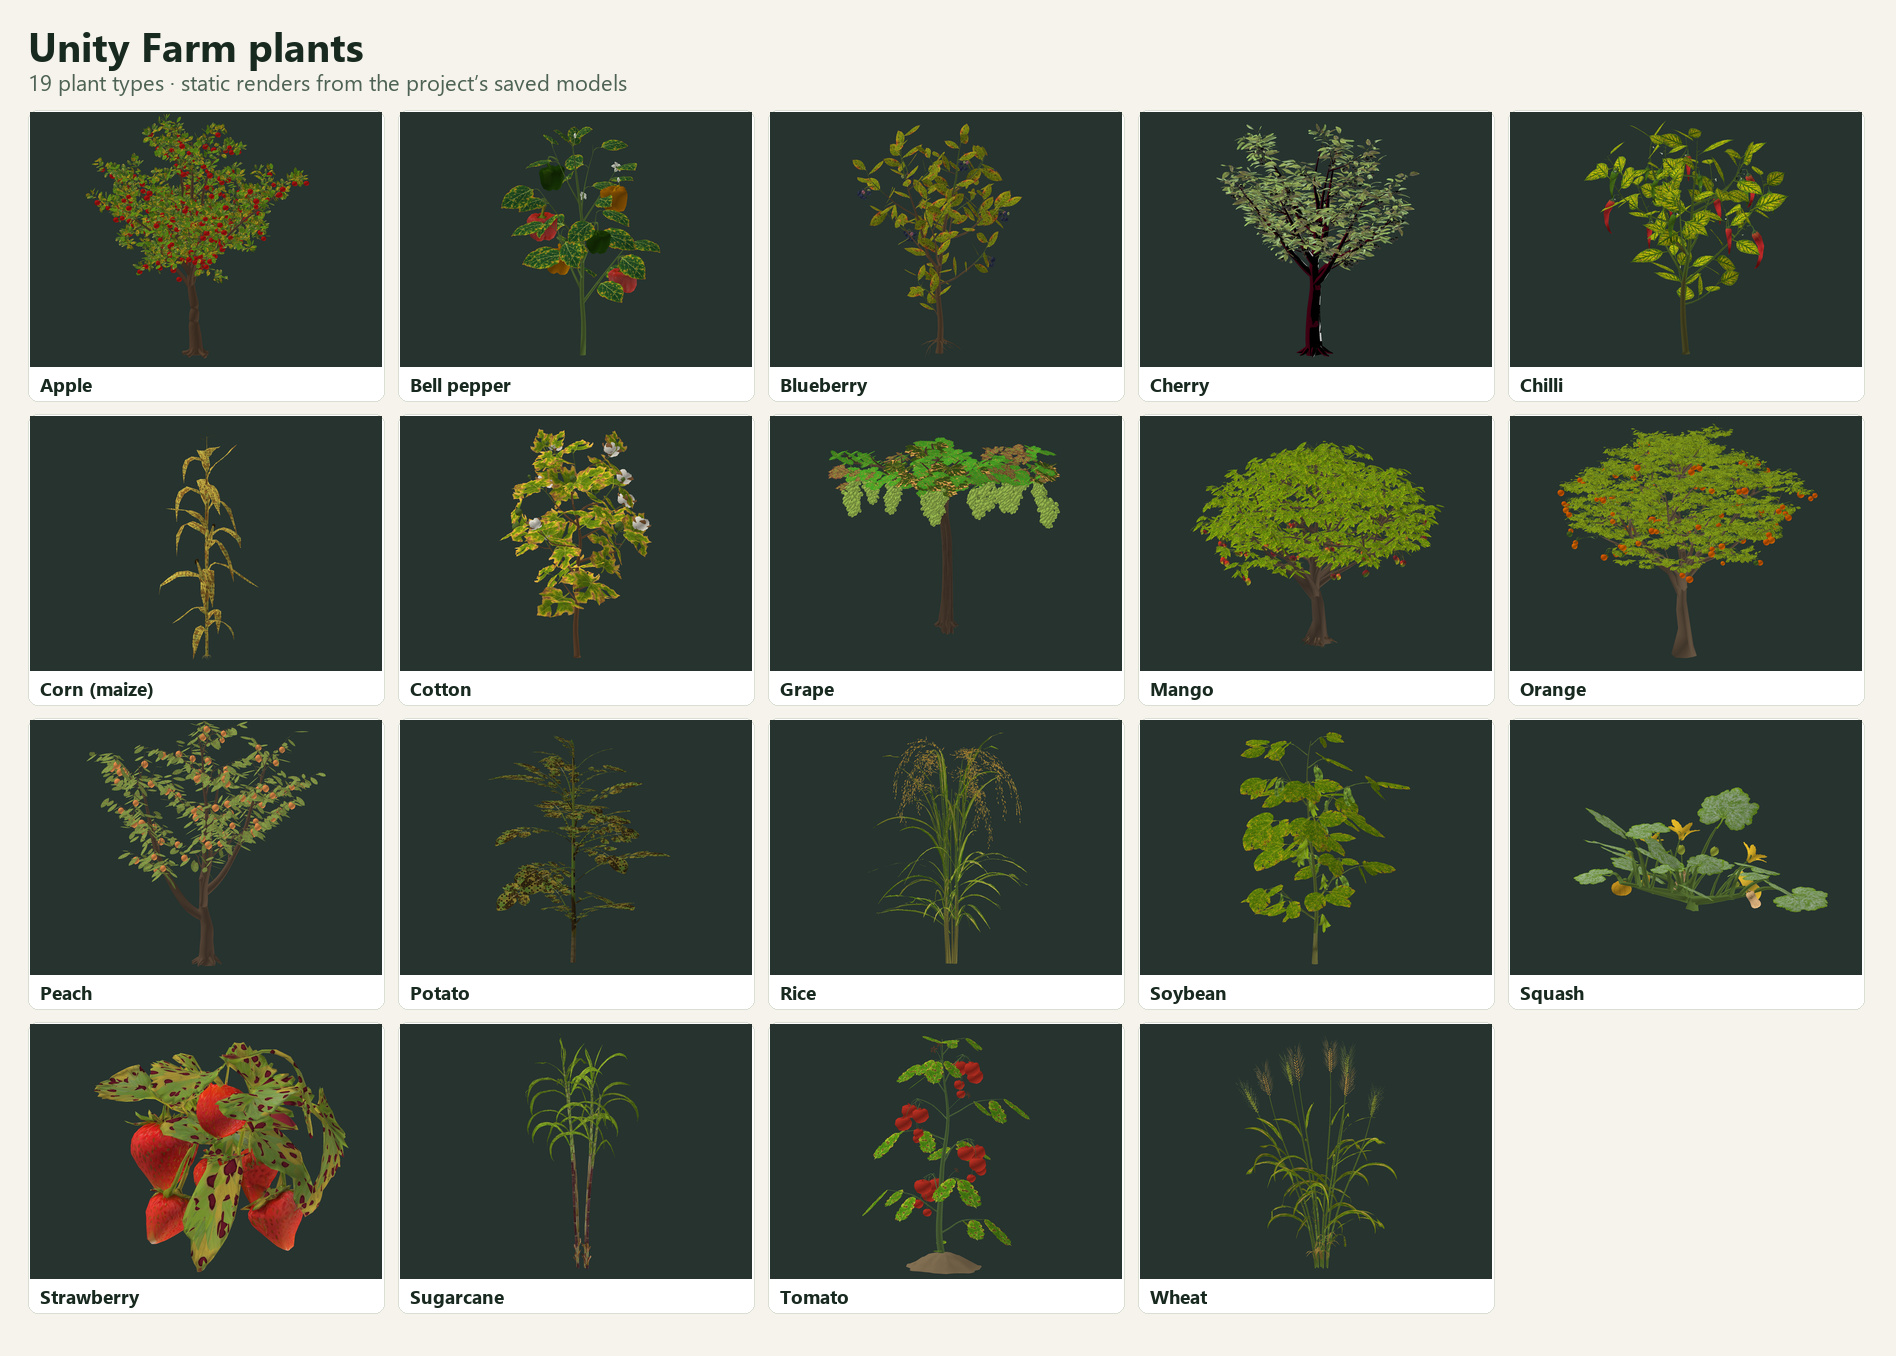
\includegraphics[width=.70\linewidth]{all-19-unity-plants.jpg}
\caption{The Unity plant collection contains 19 crop models. The team scanner covers a wider set, so only mapped cases open in VR.}\label{fig:plants}
\end{figure}

\clearpage
\section{Results and Analysis}
\subsection*{A. Unity VR checks}
All 167 tests passed in the targeted Unity EditMode run. They covered input, leaf display, treatment and recovery logic. The Android APK built successfully, and I ran the inspection, treatment and recovery sequence on a Quest headset. The headset check verified that I could complete the workflow. Frame times, comfort and learning outcomes remain open for evaluation.

\subsection*{B. Team classifier benchmark}
Top-1 accuracy is the percentage of images for which the model's first guess matches the reference label. The team tested on 4,333 PlantVillage lab photos and 236 PlantDoc field photos.

\begin{table}[!ht]
\caption{Team classifier performance on lab and field images.}\label{tab:results}
\vspace{3pt}
\begin{tabularx}{\linewidth}{@{}LN{.125\linewidth}N{.142\linewidth}N{.106\linewidth}N{.12\linewidth}@{}}
\toprule
\tabhead{Model} & \tabhead{Lab top-1} & \tabhead{Field top-1} & \tabhead{Field F1} & \tabhead{\mbox{Gap (pp)}}\\
\midrule
EfficientNet-B0, lab-only baseline & 97.1\% & 14.8\% & 0.163 & 82.2\\
EfficientNet-B0, lab and field & 97.9\% & 58.9\% & 0.593 & 39.0\\
\textbf{BioCLIP ViT-B/16, v6} & \textbf{99.4\%} & \textbf{77.1\%} & \textbf{0.770} & \textbf{22.2}\\
\bottomrule
\end{tabularx}
\vspace{3pt}
\smallnote{Field F1 is averaged across classes. The gap is lab accuracy minus field accuracy in percentage points, calculated before rounding.}
\end{table}

Field accuracy rose by 62.3 percentage points from the lab-only baseline to v6. The training data, model architecture and label set changed across runs. The latest model still scores 22.2 points higher on lab photos. Earlier error analysis found that the scanner could confuse diseases with similar symptoms, including early and late blight.

\begin{figure}[!ht]\centering
\panel{web-scan-result.jpg}{(a) Example result from the team scanner}\hfill
\panel{quest-treatment-lab.jpg}{(b) Treatment Lab running on Quest}
\caption{The scanner shows a leaf, a predicted class and an activation overlay. The headset capture shows the Unity treatment controls during the demo.}\label{fig:results}
\end{figure}

\smallnote{An earlier Quest run exposed a missing API address. The recorded treatment API run passed 160 tests, with seven deselected. Four frontend locale tests failed because a Quest installation label was missing.}

\clearpage
\section{Conclusion and Future Work}
I built a Unity VR lesson in which learners can inspect a plant, practise a treatment and follow six weeks of simulated recovery. I ran the workflow on Quest and verified that the main interactions worked. The team classifier adds a way to choose a supported case from a photo. Its field results show how much the accuracy still depends on the image conditions.

\begin{multicols}{2}
\subsection*{A. Plant reconstruction}
My mentor suggested using RGB and infrared depth cameras to capture a plant's colour and shape. These captures could produce more faithful models for Unity. The next test would compare a reconstructed plant with its source images while checking that it runs smoothly on the headset.

\subsection*{B. Field scouting}
The mentor also suggested using drone images to flag areas of a farm for inspection. A follow-up would compare those flags with observations on the ground. For the VR lesson, a learner study could test whether people recognize symptoms more accurately or choose a more appropriate response after practice.
\end{multicols}

\begingroup\small
\begin{thebibliography}{10}
\setlength{\itemsep}{2pt}
\bibitem{fao} Food and Agriculture Organization of the United Nations, \emph{Understanding the Context}, Pest and Pesticide Management. [Online]. \href{https://www.fao.org/pest-and-pesticide-management/about/understanding-the-context/en/}{FAO website}.
\bibitem{mohanty} S. P. Mohanty, D. P. Hughes, and M. Salath\'e, \textquotedblleft Using deep learning for image-based plant disease detection,\textquotedblright\ \emph{Front. Plant Sci.}, vol. 7, art. 1419, 2016. doi: \href{https://doi.org/10.3389/fpls.2016.01419}{10.3389/fpls.2016.01419}.
\bibitem{plantdoc} D. Singh \emph{et al.}, \textquotedblleft PlantDoc: A dataset for visual plant disease detection,\textquotedblright\ in \emph{Proc. ACM CoDS-COMAD}, 2020, pp. 249--253. doi: \href{https://doi.org/10.1145/3371158.3371196}{10.1145/3371158.3371196}.
\bibitem{sakha} M. M. Sakha, F. Daiber, M. Enders, C. Tieben, B. Kisliuk, and A. Kr\"uger, \textquotedblleft Enhancing plant variety discovery process with visual trait assessment in VR,\textquotedblright\ in \emph{Proc. IEEE Conf. Virtual Reality and 3D User Interfaces (VR)}, 2025, pp. 125--134. \href{https://www.dfki.de/en/web/research/projects-and-publications/publication/15771}{Publication record}.
\bibitem{bondesan} P. Bondesan, A. Canal, S. Fleury, A. Boisadan, and S. Richir, \textquotedblleft Implicit learning of professional skills through immersive virtual reality: A media comparison study,\textquotedblright\ in \emph{Proc. IEEE Conf. Virtual Reality and 3D User Interfaces (VR)}, 2025, pp. 442--449. doi: \href{https://doi.org/10.1109/VR59515.2025.00068}{10.1109/VR59515.2025.00068}.
\bibitem{cheng} K.-H. Cheng, \textquotedblleft Development of an immersive virtual reality system for learning about plants in primary education,\textquotedblright\ \emph{Educ. Technol. Res. Dev.}, vol. 72, pp. 845--867, 2024. doi: \href{https://doi.org/10.1007/s11423-023-10300-6}{10.1007/s11423-023-10300-6}.
\bibitem{bioclip} S. Stevens \emph{et al.}, \textquotedblleft BioCLIP: A vision foundation model for the tree of life,\textquotedblright\ in \emph{Proc. IEEE/CVF CVPR}, 2024, pp. 19412--19424. \href{https://openaccess.thecvf.com/content/CVPR2024/html/Stevens_BioCLIP_A_Vision_Foundation_Model_for_the_Tree_of_Life_CVPR_2024_paper.html}{CVF Open Access}.
\bibitem{plantwild} T. Wei, Z. Chen, Z. Huang, and X. Yu, \textquotedblleft Benchmarking in-the-wild multimodal disease recognition and a versatile baseline,\textquotedblright\ in \emph{Proc. ACM Multimedia}, 2024, pp. 1593--1601. doi: \href{https://doi.org/10.1145/3664647.3680599}{10.1145/3664647.3680599}.
\bibitem{eff} M. Tan and Q. V. Le, \textquotedblleft EfficientNet: Rethinking model scaling for convolutional neural networks,\textquotedblright\ in \emph{Proc. ICML}, vol. 97, 2019, pp. 6105--6114. \href{https://proceedings.mlr.press/v97/tan19a.html}{PMLR}.
\bibitem{repo} CropScan XR team, \emph{VR Plant Treatment}, project source and local benchmark and test records, 2026. \href{https://github.com/bhargavm-iiits/VR-Plant-Treatment}{Project repository}.
\end{thebibliography}
\endgroup
\end{document}
